%%%%%%%%%%%%%%%%%%%%%%%%%%%%%%%%%%%%%%%%%
% Focus Beamer Presentation
% LaTeX Template
% Version 1.0 (8/8/18)
%
% This template has been downloaded from:
% http://www.LaTeXTemplates.com
%
% Original author:
% Pasquale Africa (https://github.com/elauksap/focus-beamertheme) with modifications by
% Vel (vel@LaTeXTemplates.com)
%
% Template license:
% GNU GPL v3.0 License
%
% Important note:
% The bibliography/references need to be compiled with bibtex.
%
%%%%%%%%%%%%%%%%%%%%%%%%%%%%%%%%%%%%%%%%%

%----------------------------------------------------------------------------------------
%	PACKAGES AND OTHER DOCUMENT CONFIGURATIONS
%----------------------------------------------------------------------------------------

\documentclass{beamer}
\usepackage[ngerman]{babel}
\usepackage{xcolor}

\definecolor{hmred}{RGB}{251, 86, 85}
\usepackage{leftidx}
\usepackage{filecontents}
\usepackage{graphicx}
\usepackage{tikz}
\usepackage{pgfplots}
\usepackage{amsthm}
\usepackage{amsmath}
\usepackage{amssymb}
\usepgfplotslibrary{groupplots}
\usepackage{amsmath}
\DeclareMathOperator*{\argmax}{arg\,max}
\DeclareMathOperator*{\argmin}{arg\,min}

\usetheme{focus} % Use the Focus theme supplied with the template
% Add option [numbering=none] to disable the footer progress bar
% Add option [numbering=fullbar] to show the footer progress bar as always full with a slide count

% Uncomment to enable the ice-blue theme
%\definecolor{main}{RGB}{92, 138, 168}
%\definecolor{background}{RGB}{240, 247, 255}

%------------------------------------------------

\usepackage{booktabs} % Required for better table rules

% [noframenumbering] frame without number
% [plain] frame without header
%----------------------------------------------------------------------------------------
%	 TITLE SLIDE
%----------------------------------------------------------------------------------------

\title{CART-Klassifikator}

\subtitle{Pattern Matching \& Machine Learning}

\author{F. Freter, E. Kirchberger,\\S. Symhoven \& J. Wustl}

\institute{Sommersemester 2023}

\titlegraphic{
\includegraphics[scale=0.305]{Images/hmlogo.png} \\ \textcolor{hmred}{Hochschule München \\ University of Applied Sciences \\ Fakultät für
Informatik und Mathematik}} % Optional title page image, comment this line to remove itt

\date{20. Juni 2022}


%------------------------------------------------

\begin{document}



%------------------------------------------------

\begin{frame}
	\maketitle % Automatically created using the information in the commands above
\end{frame}

%------------------------------------------------

\begin{frame}{Inhalt}
	\tableofcontents % Automatically created using the information in the commands above
\end{frame}


%----------------------------------------------------------------------------------------
%	 SECTION 1
%----------------------------------------------------------------------------------------


\section{Training und Aufbau des Baumes}
 
\begin{frame}{CART: Classification And Regression Trees}
	\begin{columns}
		\column{0.5\textwidth}
			\textbf{CART-Algorithmen}: sind Binary-Decisson Tree Verfahren, welches für \textbf{Klassifizierung} (kategorisch) und \textbf{Regression} (kontinuierlich) verwendet werden kann.
			
			\begin{alertblock}{Classification Trees}
				Im Folgenden fokussieren wir uns auf die  \textbf{Classification Trees}.
			\end{alertblock}
			
		\column{0.5\textwidth}
			\begin{figure}
				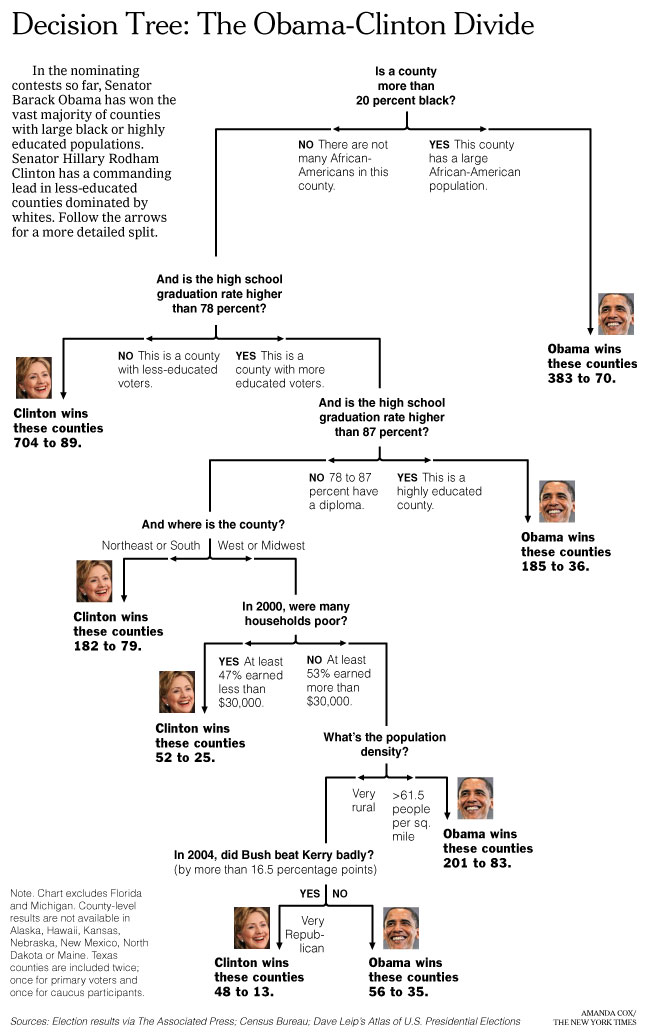
\includegraphics[height=7cm]{Images/0416-nat-subOBAMA.jpg}
				\caption{Decision Tree \cite{hastie_tibshirani_friedman}}
			\end{figure}
	\end{columns}
		
	
\end{frame}

\begin{frame}{Aufbau eines Classification Trees}

	\begin{columns}
		\column{0.5\textwidth}
			\begin{itemize}
				\item {\textbf{Root Node}: Startpunkt, enthält alle Daten und startet die Unterteilung (basierend auf Merkmalen mit Informationsgewinn).}
				\item {\textbf{Decision Node}: Teilt Daten weiter auf (basierend auf übrigen Merkmalen).}
				\item {\textbf{Leaf Node}: Endpunkte repräsentieren finale Vorhersagen (basierend auf Merkmalen des gegebenen Datenpunkts. Hier sind keine weiteren sinnvollen Teilungen mehr möglich).}
			\end{itemize}	
			
		\column{0.5\textwidth}
			\begin{figure}
			
				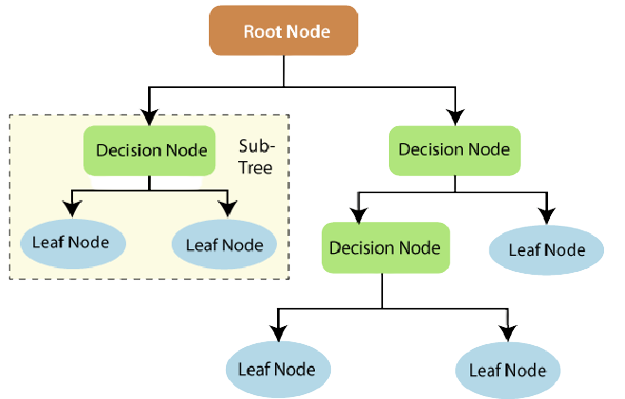
\includegraphics[width=\linewidth]{Images/tree.png}
				\caption{Decision Tree \cite{Charbuty2021ClassificationBO}}
			\end{figure}
			
			\pause
			\begin{alertblock}{Ziel}
				Optimale Vorhersagen auf Basis von Eingangsmerkmalen.			
			\end{alertblock}
	\end{columns}

\end{frame}

\begin{frame}{Allgemeine Strategie}
	\textbf{Allgemeine Strategie}: Eingangsdaten werden in $P$ disjunkte Regionen $R_1,\dots,R_P$ aufgeteilt. 
	wobei jede Region $R_p$ eine Entscheidungsklasse $Y_p$ repräsentiert. 
 \textbf{Binary Splitting}, Beispiel: $x_i <= a$ \vspace{0.25cm}
	
	\begin{columns}
		\column{0.5\textwidth}
				\textbf{Trainings Methode}:
				\begin{itemize}
					\item {Aufteilung des Ausgangsraums $R$ in $R_1$ und $R_2$}
					\item{Suche nach der besten Aufteilung für $R_1$ und $R_2$}
					\item{Wiederhole für alle erzeugten Regionen}
				\end{itemize}
			
		\column{0.43\textwidth}
			\begin{figure}
				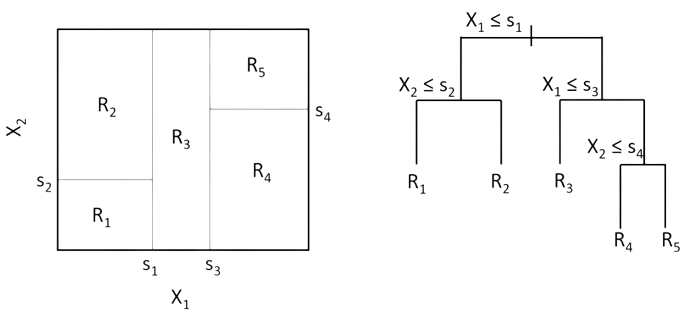
\includegraphics[width=\linewidth]{Images/split.png}
				\caption{Rekursive Teilung \cite{hastie_tibshirani_friedman}}
			\end{figure}
	\end{columns}
\end{frame}

\begin{frame}{Vorgehen bei Klassifikation}
	
	\begin{figure}
		
\includegraphics[width=\linewidth]{Images/training.png}
		\caption{Training- und Validation Set \cite{machine-learning}}
	\end{figure}
	
	\begin{itemize}
		\item Teile das Datenset in ein Lern- und ein Test-Set eingeteilt.
		\item Das Lern-Set wird zusätzlich in ein Training- und Validierungs-Set gesplittet.
		\item Baue Klassifkationsbaum auf Trainingsmenge $\mathcal{D}_T$ und führe Klassifizierung auf Validierungsmenge durch.
		\item Vergleiche tatsächliche Klassen mit vorhergesagten Klassen und wähle den Baum mit der besten Performance.
		\item Messe finale Performance auf dem Test-Set.
	\end{itemize}

\end{frame}

\begin{frame}{Vorgehen bei Klassifikation}

Um ein neues Sample $X$ zu klassifizieren:
	\begin{itemize}
		\item Test der Attribute von $X$ um die zutreffende Region zu finden für die Klassenverteilung $y_r = (y_{c_1}, \ldots, y_{c_k})$.
		\item Die Wahrscheinlichkeit das ein Punkt $X \in \mathcal{R}$ zu einer Gruppe gehört, ist definiert durch
			\[p(y = c | \mathcal{R}) = \frac{y_c, \mathcal{R}}{\sum_{c_i \in C} y_{c_i}, \mathcal{R}}.\]
		\item Ein neues Sample bekommt die Zuteilung welche am häufigsten in der jeweiligen Region ist.
			\[\hat{y} = \argmax_c p(y = c | x) = \argmax_c p(y = c | \mathcal{R}) = \argmax_c y_{c,\mathcal{R}}\]
	\end{itemize}
\end{frame}


%----------------------------------------------------------------------------------------
%	 SECTION 2
%----------------------------------------------------------------------------------------

\section{Bewertungsmaße für einen Split}
%------------------------------------------------

\begin{frame}{Bewertungsmaße: Gini-Index, Informationsgewinn \& Missclassification Error}
	\begin{itemize}
		\item{\textbf{Gini-Index}}
		\begin{itemize}
			\item Maß der Unreinheit einer Gruppe
			\item $i_G (t) = 1 - \sum_{i=1}^k \pi_i^2$, wobei $\pi_i$ die Wkt. der Klasse $i$ ist.
			\item \textbf{Ziel}: Minimierung des gewichteten Gini-Indexes.
		\end{itemize}
		\item{\textbf{Informationsgewinn: Entropy}}
		\begin{itemize}
			\item Reduktion der Entropie durch den Split
			\item $IG = H(parent) - \sum_{j=1}^m \frac{n_j}{n} H(child_j)$, wobei $H$ die Entropie ist.
			\item \textbf{Ziel}: Maximierung des Informationsgewinns.
		\end{itemize}
		\item{\textbf{Missclassification Error}}
		\begin{itemize}
			\item {Der Misclassification Error (ME) ist ein Maß für die Fehlklassifizierung.}
			\item $i_E (t) = 1 - \max_c p(y = c | t)$
			\item {ME kann als Bewertungsmaß für die Baumkonstruktion verwendet werden.}
		\end{itemize}
	\end{itemize}
\end{frame}

\begin{frame}{Gini-Index}
	Misst, wie oft eine zufällig ausgewählte Instanz falsch klassifiziert würde, wenn sie gemäß der Klassenverteilung zufällig klassifiziert wird.
	
	\begin{itemize}
		\item Die Gini-Unreinheit ist ein Wert zwischen 0 (vollständig rein, alle Elemente gehören zur gleichen Klasse) und 1 (maximal unrein, gleichmäßige Verteilung der Klassen).
		\item Die Gini-Unreinheit für einen Knoten $t$ mit $K$ Klassen kann wie folgt berechnet werden:
		\[
		i_G (t) = \sum_{c_i \in C} \underbrace{\pi_{c_i}}_{\substack{\text{Wahrscheinlichkeit,} \\ \text{ein Element auszuwählen}}} \cdot \underbrace{(1 - \pi_{c_i})}_{\substack{\text{Wahrscheinlichkeit,} \\ \text{dass es falsch} \\ \text{klassifiziert wird}}}
		\]
	\end{itemize}
	\end{frame}
	
\begin{frame}{Der beste Split}
	\begin{alertblock}{Problem: Wie finde ich den besten Split?}
		Direkte Optimierung ist schwer umsetzbar, da die iterative Überprüfung aller Bäume bei komplexeren Daten schnell explodiert.
		\\\vspace{0.5cm}
		
		
		Mögliche Lösung:\\ \vspace{0.5cm}
		
		
		\textbf{Greedy Heuristic}: Bei jedem Schritt wird die aktuell optimale Entscheidung getroffen
	
	\end{alertblock}
	
	\end{frame}
	
	
	\begin{frame}{Greedy Heuristic}
	
	Hierbei wird eine Node aufgeteilt, wenn sie den Misclassification Error (ME) $i_E$ an Node $t$ verbessert.
	   \[
		   i_E (t) = 1 - \max_c p(y = c | t)
	   \]
	
	Die Verbesserung bei Durchführung eines Splitts $s$ von $t$ zu $t_R$ und $t_L$ für $i(t) = i_E (t) $ ist wie folgt definiert: 
	\[
		\Delta i(s, t) = i(t) - p_L \cdot i(t_L) - p_R \cdot i(t_R)
	\]	
	
	\end{frame}
	\begin{frame}{Probleme mit Misclassification Error}
	\textbf{Problem 1:} Kein Splitt durchgeführt bei $i_E (t) = \frac{40}{200}$, obwohl verbesserte Klassifikation möglich, durch Kombination von Tests.
	 \begin{align*}
		 x_1 \leq 5&: p_L \cdot i_E (t_L) - p_R \cdot i_E (t_R) = \frac{40}{200} \\
		x_2 \leq 3&: p_L \cdot i_E (t_L) - p_R \cdot i_E (t_R) = \frac{40}{200} \\
	 \end{align*}
	\textbf{Problem 2:}
	Schlechte Sensitivität zur Veränderung der Klassenwahrscheinlichkeiten.
	Verteilung vor Split: $(400, 400)$
	 \begin{align*}
		 \text{Split } a &: \{(100,300), (300,100)\} \rightarrow i_E (t, a) = 0.25 \\
		\text{Split } b &: \{(200,400), (200,0)\} \rightarrow i_E (t, b) = 0.25 \\
	 \end{align*}
	 \textbf{Lösung}: Ein Kriterium welches als Maß für die Reinheit der Klassenverteilung an Node $t$ verwendet werden kann.
	\end{frame}
	

%----------------------------------------------------------------------------------------
%	 SECTION 3
%----------------------------------------------------------------------------------------

\section{Overfitting und Pruning}

\begin{frame}{Overfitting in Decision Trees}
Daten werden rekursiv aufgeteilt und lassen den DT dadurch wachsen. Wann sollte man das Wachstum stoppen um overfitting zu vermeiden?\\
\textbf{Mögliche Stop- (oder Pruning-) Kriterien:}
\begin{itemize}
\item Verteilung im Ast ist rein, d.h. i(t) = 0
\item Maximale Tiefe erreicht
\item Anzahl der Proben in jedem Ast unterhalb eines bestimmten Schwellenwerts $t_n$
\item Nutzen der Aufteilung ist unterhalb eines bestimmten Schwellenwerts $\Delta i(s,t) < t\Delta$
\item Genauigkeit auf dem Validierungsset
\item {\textbf{Ziel}: Erstellung eines Modells, das gut auf neue, ungesehene Daten verallgemeinert und somit Overfitting vermeidet.}
\end{itemize}
\end{frame}

\begin{frame}{Pruning Methods}
Alternativ kann der Baum zunächst vollständig wachsen und anschließend beschnitten werden (\textbf{Post-Pruning}).
 \begin{alertblock}{Verschiede Pruning-Methoden:}
\begin{itemize}
\item Reduced Error Pruning
\item Minimum Description Length Pruning
\item Cost-Complexity Pruning

\end{itemize}

\end{alertblock}
\end{frame}

\begin{frame}{Cost-Complexity Pruning}
	\begin{itemize}
		\item {\textbf{Ziel}: Verhindern von Overfitting durch Entfernen von Zweigen, die wenig zur Vorhersageleistung beitragen}
		\item {\textbf{Kostenkomplexitätspruning}: Gleichgewicht zwischen Baumgröße und Trainingsfehler}
		\item \textbf{Kostenkomplexitätskriterium}: \[C_{\alpha}(T) = C(T) + \alpha|T|, \, mit\]
		\begin{itemize}
			\item $C(T)$ ist der Misclassification Error des Baumes $T$.
			\item $|T|$ ist die Anzahl der terminalen Knoten des Baumes $T$.
			\item $\alpha$ ist ein Komplexitätsparameter, der die Präferenz zwischen Baumgröße und Trainingsfehler steuert.
		\end{itemize}
		\item Durch Variieren von $\alpha$ kann eine Sequenz optimaler Bäume ermittelt werden.
		\item Kreuzvalidierung kann verwendet werden, um den optimalen Wert von $\alpha$ zu bestimmen.
	\end{itemize}
\end{frame}

%----------------------------------------------------------------------------------------
%	 SECTION 4
%----------------------------------------------------------------------------------------




%----------------------------------------------------------------------------------------
%	 SECTION 5
%----------------------------------------------------------------------------------------

\section{Vor- und Nachteile}

\begin{frame}
	\begin{columns}[T, onlytextwidth]
		\column{0.5\textwidth}
			\textbf{Vorteile}:
			\begin{itemize}
				\item leicht zu trainieren
				\item leicht zu interpretieren
				\item einfach zu visualisieren
				\item können mit verschiedenen Prädiktoren umgehen \\$\rightarrow$ keine Dummies erforderlich
			\end{itemize}
		
		\column{0.5\textwidth}
			\textbf{Nachteile}:
			\begin{itemize}
				\item nicht die besten Lerner
				\item reagieren empfindlich auf sich ändernde Trainingsdaten
				\item werden von den oben genannten Splits dominiert \\$\rightarrow$ erster Split beeinflusst stark die Form des gesamten Baums
			\end{itemize}
	\end{columns}
\end{frame}

%----------------------------------------------------------------------------------------
%	 SECTION 6
%----------------------------------------------------------------------------------------

\section{Verbesserungsmöglichkeiten \& Ausblick}

\begin{frame}
		\begin{itemize}
			\item\textbf{Stacking}: Ensemble-Lern-Technik. Mehrere CART-Modelle kombiniert werden. Ausgaben der einzelnen Modelle  werden als Eingabe für ein Meta-Modell verwendet.
			\item\textbf{Bayesian Model Averaging}: Modellselektion. Mehrere Modelle auf der Grundlage von Bayes'schen Wahrscheinlichkeiten kombiniert werden.
			\item\textbf{Bagging}: Ensemble-Lern-Technik. Mehrere CART-Modelle werden auf unterschiedlichen Stichproben der Daten trainiert.
			\item\textbf{Random Forests}: Ensemble-Lern-Modell. Besteht aus vielen unkorrelierten Entscheidungsbäumen, die auf zufälligen Untergruppen der Daten trainiert werden.
			\item\textbf{Boosting}: Ensemble-Lern-Technik. Sequentielle Anordnung von schwachen CART-Modellen, wobei jeder Baum versucht, die Fehler des vorherigen Baums zu korrigieren.
		\end{itemize}
\end{frame}


%----------------------------------------------------------------------------------------
%	 CLOSING/SUPPLEMENTARY SLIDES
%----------------------------------------------------------------------------------------

\appendix

\begin{frame}[allowframebreaks]{References}
	\bibliography{references.bib}
	\nocite{*}
	\bibliographystyle{plain}
\end{frame}

\begin{frame}[focus]

	Fragen, Kritik oder Anregungen?
	
\end{frame}

%----------------------------------------------------------------------------------------

\end{document}
